\documentclass[12pt]{article}
\usepackage[utf8]{inputenc}

\usepackage{lmodern}

\usepackage{enumitem}
\usepackage[margin=2cm]{geometry}

\usepackage{amsmath, amsfonts, amssymb}
\usepackage{graphicx}
%\usepackage{subfigure}
\usepackage{tikz}
\usepackage{pgfplots}
\usepackage{multicol}

\usepackage{comment}
\usepackage{url}
\usepackage{calc}
\usepackage{subcaption}
\usepackage[indent=0pt]{parskip}
\usepackage{animate}

\usepackage{array}
\usepackage{blkarray,booktabs, bigstrut}
\usepackage{bigints}

\pgfplotsset{compat=1.16}

% MATH commands
\newcommand{\ga}{\left\langle}
\newcommand{\da}{\right\rangle}
\newcommand{\oa}{\left\lbrace}
\newcommand{\fa}{\right\rbrace}
\newcommand{\oc}{\left[}
\newcommand{\fc}{\right]}
\newcommand{\op}{\left(}
\newcommand{\fp}{\right)}

\newcommand{\bi}{\mathbf{i}}
\newcommand{\bj}{\mathbf{j}}
\newcommand{\bk}{\mathbf{k}}
\newcommand{\bF}{\mathbf{F}}

\newcommand{\mR}{\mathbb{R}}

\newcommand{\ra}{\rightarrow}
\newcommand{\Ra}{\Rightarrow}

\newcommand{\sech}{\mathrm{sech}\,}
\newcommand{\csch}{\mathrm{csch}\,}
\newcommand{\curl}{\mathrm{curl}\,}
\newcommand{\dive}{\mathrm{div}\,}

\newcommand{\ve}{\varepsilon}
\newcommand{\spc}{\vspace*{0.5cm}}

\DeclareMathOperator{\Ran}{Ran}
\DeclareMathOperator{\Dom}{Dom}

\newcommand{\exo}[1]{\noindent\textcolor{red}{\fbox{\textbf{Problem {#1}}}\hrulefill}\\}
\newcommand{\qu}[4]{\noindent\textcolor{#4}{\fbox{\textbf{Section {#1} | Problem {#2}}} \hrulefill{{\fbox{\textbf{{#3} Points}}}}\\}}

\newcommand{\semester}{Spring 2023}

\newcommand{\CVup}{%

\begin{tikzpicture}
\draw[black, <->, >=latex] (-0.33, 0.5) .. controls (-0.125, 0) and (0.125, 0) .. (0.33, 0.5);
\end{tikzpicture}}

\newcommand{\CVupInc}{%
\begin{tikzpicture}
\draw[black, ->, >=latex] (0,0) .. controls (0.2, 0) and (0.4, 0.2) .. (0.5, 0.5);
\end{tikzpicture}}

\newcommand{\CVupDec}{%
\begin{tikzpicture}[rotate=270]
\draw[black, ->, >=latex] (0,0) .. controls (0.2, 0) and (0.4, 0.2) .. (0.5, 0.5);
\end{tikzpicture}}

\newcommand{\CVdown}{%
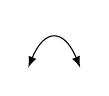
\begin{tikzpicture}
\draw[black, <->, >=latex] (-0.33, -0.5) .. controls (-0.125, 0) and (0.125, 0) .. (0.33, -0.5);
\end{tikzpicture}}

\newcommand{\CVdownInc}{%
\begin{tikzpicture}
\draw[black, ->, >=latex] (-0.5, -0.5) .. controls (-0.5, -0.3) and (-0.5, -0.1) .. (0,0);
\end{tikzpicture}}

\newcommand{\CVdownDec}{%
\begin{tikzpicture}[rotate=-90]
\draw[black, ->, >=latex] (-0.5, -0.5) .. controls (-0.5, -0.3) and (-0.5, -0.1) .. (0,0);
\end{tikzpicture}}

\begin{document}
	\noindent \hrulefill \\
	MATH-241 \hfill Pierre-Olivier Paris{\'e}\\
	Solutions Section 4-4 \hfill \semester \\\vspace*{-1cm}
	
	\noindent\hrulefill
	
	\spc	
	
	\exo{5}
	\\
	We have
		\begin{align*}
		\int (x^{1.3} + 7x^{2.5}) \, dx = \int x^{1.3} \, dx + 7 \int x^{2.5} \, dx = \frac{x^{1.3 + 1}}{1.3 + 1} + 7 \frac{x^{2.5 + 1}}{2.5 + 1} + C = \frac{x^{2.3}}{2.3} + 7 \frac{x^{3.5}}{3.5} + C .
		\end{align*}
		
	\spc
	
	\exo{6}
	\\
	We can write $\sqrt[4]{x^5} = x^{5/4}$ and therefore
		\begin{align*}
		\int \sqrt[4]{x^5} \, dx = \frac{x^{5/4}}{5/4} + C = \frac{4}{5} x^{5/4} + C .
		\end{align*}
		
	\spc
	
	\exo{10}
	\\
	We have
		\begin{align*}
		\sqrt{t} (t^2 + 3t + 2) = t^{5/2} + 3 t^{3/2} + 2t^{1/2}
		\end{align*}
	and therefore
		\begin{align*}
		\int \sqrt{t} (t^2 + 3t + 2) \, dt = \int t^{5/2} \, dt + 3 \int t^{3/2} \, dt + 2 \int t^{1/2} \, dt = \frac{2}{7} t^{7/2} + \frac{6}{5} t^{5/2} + \frac{4}{3} t^{3/2} + C .
		\end{align*}
	
	\spc
	
	\exo{11}
	\\
	
	We have
		\begin{align*}
		\frac{1 + \sqrt{x} + x}{\sqrt{x}} = \frac{1}{\sqrt{x}} + 1 + \sqrt{x} = x^{-1/2} + 1 + x^{1/2} .
		\end{align*}
	Therefore, 
		\begin{align*}
		\int \frac{1 + \sqrt{x} + x}{\sqrt{x}} \, dx = \int x^{-1/2} \, dx + \int \, dx + \int x^{1/2} \, dx = 2 x^{1/2} + x + \frac{2}{3} x^{3/2} + C .
\end{align*}

	\spc
	
	\exo{14}
	\\
	We have
		\begin{align*}
		\sec t (\sec t + \tan t) = \sec^2 t + \sec t \tan t .
		\end{align*}	
	Therefore,
		\begin{align*}
		\int \sec t (\sec t + \tan t) \, dt = \int \sec^2 t \, dt + \int \sec t \tan t \, dt = \tan t + \sec t + C .
		\end{align*}	
		
	\spc
	
	\exo{15}
	\\
	We have
		\begin{align*}
		\frac{1 - \sin^3 t}{\sin^2 t} = \frac{1}{\sin^2 t} - \sin t = \csc^2 t - \sin t .
		\end{align*}	
	Therefore,
		\begin{align*}
		\int \frac{1 - \sin^3 t}{\sin^2 t} \, dt = \int \csc^2 t \, dt - \int \sin t \, dt = -\cot t + \cos t + C .
\end{align*}	

	\spc
	
	\exo{18}
	\\
	We have
		\begin{align*}
		(1 - x^2)^2 = 1 - 2x^2 + x^4
		\end{align*}
	and so
		\begin{align*}
		\int (1 - x^2)^2 \, dx = \int \, dx - 2 \int x^2 \, dx + \int x^4 \, dx = x - \frac{2}{3} x^3 + \frac{x^5}{5} + C .
		\end{align*}
	
	Here is the graph of several antiderivatives with different constants $C$.
	
		\begin{figure}[h]
		\centering
		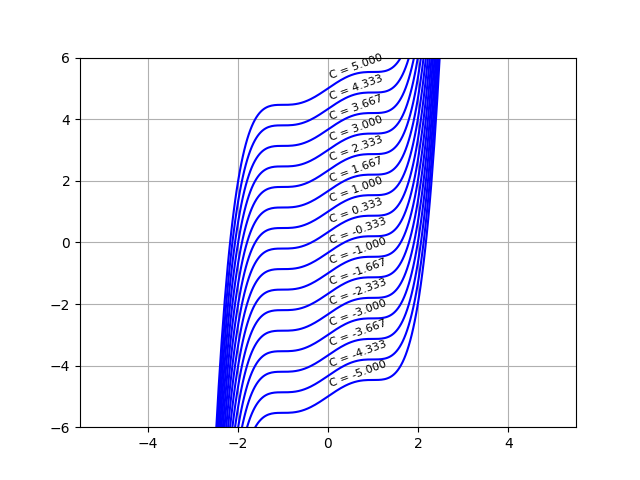
\includegraphics[scale=0.68]{exo18.png}
		\end{figure}
		
	\newpage
	
	\exo{41}
	\\
	When $x \leq 0$, we have
		\begin{align*}
		x - 2|x| = x + 2x = 3x
		\end{align*}			
	and when $x \geq 0$, we have
		\begin{align*}
		x - 2|x| = x - 2x = -x .
		\end{align*}
	Therefore, the integral is	
		\begin{align*}
		\int_{-1}^2 (x - 2|x|) \, dx = \int_{-1}^0 3x \, dx - \int_0^3 x \, dx &= 3 \big( \frac{0^2 - (-1)^2}{2} \big) - \big( \frac{3^2 - 0^2}{2} \big) \\
		&= -\frac{3}{2} - \frac{9}{2} = -6 .
\end{align*}											
	
	\exo{58}
	\begin{enumerate}[label=(\alph*)]
	\item The velocity is given by 
		\begin{align*}
		v(t) =  \int 2t + 3 \, dt = t^2 + 3t + C .
		\end{align*}
	Now, $v(0) = -4$, so $C = -4$. We then get 
		\begin{align*}
		v(t) = t^2 + 3t - 4 = (t + 4 ) (t - 1) .
		\end{align*}
	\item The distance travelled during the interval is given by
		\begin{align*}
		\int_0^{3} |v(t)| \, dt .
		\end{align*}
	The function $v(t) = (t + 4)(t - 1)$ and therefore
		\begin{align*}
		|v(t)| = \left\{ \begin{matrix}
		- (t^2 + 3t - 4 ) & \text{ if } 0 \leq t \leq 1 \\
		t^2 + 3t - 4 & \text{ if } 1 < t \leq 3 .
		\end{matrix} \right.
		\end{align*}
	We then obtain
		\begin{align*}
		\int_0^3 |v(t)| \, dt &= \int_0^1 -t^2 - 3t + 4 \, dt + \int_1^3 t^2 + 3t - 4 \, dt \\
		&= \left. \big( -\frac{t^3}{3} - \frac{3}{2} t^2 + 4t \big) \right|_0^1 + \left. \big( \frac{t^3}{3} + \frac{3}{2} t^2 - 4t \big) \right|_1^3 \\
		&= \frac{89}{6}
		\end{align*}
	Therefore, the total distance traveled is $\frac{89}{6} \approx 14.8333$ meters.
	\end{enumerate}
	
\end{document}